\documentclass{beamer}

\usepackage[english]{babel}
\usepackage{multirow}
\usepackage{amsmath,amsthm}
\usepackage{amsfonts}
\usepackage{xkeyval}
\usepackage{graphics}
\usepackage{url}
\usepackage[lined,boxed,linesnumbered]{algorithm2e}
\usepackage{CJKutf8} %支持中文

\mode<presentation>
{
  %\usetheme{}
  %\usecolortheme{beaver}
  % 可供选择的主题参见 beameruserguide.pdf, 第 134 页起
  % 无导航条的主题: Bergen, Boadilla, Madrid, Pittsburgh, Rochester;
  % 有树形导航条的主题: Antibes, JuanLesPins, Montpellier;
  % 有目录竖条的主题: Berkeley, PaloAlto, Goettingen, Marburg, Hannover;
  % 有圆点导航条的主题: Berlin, Dresden, Darmstadt, Frankfurt, Singapore, Szeged;
  % 有节与小节导航条的主题: Copenhagen, Luebeck, Malmos, Warsaw
  %\setbeamercovered{transparent}
  % 如果取消上一行的注解 %, 就会使得被覆盖部分变得透明(依稀可见)
}
\definecolor{kured}{RGB}{240,45,104}
\definecolor{kuredlys}{RGB}{219,49,100}
\definecolor{kuredlyslys}{RGB}{249,90,138}
\definecolor{kuredlyslyslys}{RGB}{230,118,152}
\setbeamercovered{transparent} %设置半透明化尚未出现的内容
\mode<presentation>
{
  \usetheme{Antibes}
  \usecolortheme[named=kured]{structure}
  \useinnertheme{circles}
  \usefonttheme[onlymath]{serif}
  \setbeamercovered{transparent}
  \setbeamertemplate{blocks}[rounded][shadow=true]
}


\logo{
\includegraphics[scale=0.08]{images/HUSTLogo}}%Logo of the presentation
\title{Co-Regularized Hashing for Multimodal Data}
\subtitle{Yi Zhen,Dit-Yan Yeung-NIPS2012}
\author{Yunfei Wang}
\institute{Department of Computer Science \& Technology \\ Huazhong University of Science \& Technology}
\date{\today}

\begin{document}

\begin{CJK*}{UTF8}{gbsn} %中文支持

\begin{frame}
\titlepage
\end{frame}


\begin{frame}\frametitle{Table of contents}
\tableofcontents
\end{frame}

\section{Co-Regularized Hashing}
\subsection{Objective Function}
\begin{frame}[allowframebreaks]\frametitle{Objective Function}
\begin{block}{Notations}
Two data sets from two modalities:$\{x_i\in\mathcal{X}\}_{i=1}^I$,$\{y_j\in\mathcal{Y}_{j=1}^J\}$.\\
$N$ inter-modality pairs: $\Theta=\{(x_{a1},y_{b1}),\cdots,(x_{aN},y_{bN})\}$.\\
Pair label $s_n=1$($x_{an}$ and $y_{bn}$ are similar);$s_n=0$(otherwise).
\end{block}
Two linear hash functions for each bit of hash codes:
\begin{displaymath}
f(x)=sgn(w_x^Tx)
\end{displaymath}
\begin{displaymath}
g(y)=sgn(w_y^Ty)
\end{displaymath}
where $sgn(\cdot)$ denotes the sign function,$w_x$ and $w_y$ are projection vectors mapping similar points to the same hash bins and dissimilar points to different bins.

\textcolor{red}{Intra-modality loss terms:}
\begin{displaymath}
\ell_i^x=[1-f(x_i)(w_x^Tx_i)]_+=[1-|w_x^Tx_i|]_+
\end{displaymath}
\begin{displaymath}
\ell_j^y=[1-g(y_j)(w_y^Ty_j)]_+=[1-|w_y^Ty_j|]_+
\end{displaymath}
where $[a]_+$ equals $a$ if $a\geq 0$ and $0$ otherwise.

\textcolor{red}{Intra-modality loss terms:}
\begin{displaymath}
\ell_n^\ast =s_nd_n^2+(1-s_n)\tau(d_n)
\end{displaymath}
where $d_n=w_x^Tx_{an}-w_y^Ty_{bn}$,$\tau(d)$ requires the similar inter-modality points have small distance after projection and the dissimilar ones have large distance.

The SCISD(smoothly clipped inverted squared deviation) function:
\begin{displaymath}
\tau(d)=
  \begin{cases}
    -\frac{1}{2}d^2+\frac{a\lambda^2}{2}, & |d|\leq\lambda \\
    \frac{d^2-2a\lambda|d|+a^2\lambda^2}{2(a-1)}, & \lambda<|d|\leq a\lambda \\
    0, & a\lambda<|d|
  \end{cases}
\end{displaymath}
where $a$ and $\lambda$ are user-specified parameters.SCISD function penalizes projection vectors resulting in small distance between dissimilar points after projection.

\textcolor{blue}{Express SCISD function as a difference of two convex functions:$\tau(d)=\tau_1(d)-\tau_2(d)$} where
\begin{columns}
\begin{column}{0.6\textwidth}
\begin{displaymath}
\tau_1(d)=
\begin{cases}
0,& |d|\leq\lambda\\
\frac{ad^2-2a\lambda|d|+a\lambda^2}{2(a-1)},& \lambda<|d|\leq a\lambda\\
\frac{1}{2}d^2-\frac{a\lambda^2}{2},& a\lambda<|d|
\end{cases}
\end{displaymath}
\end{column}
\begin{column}{0.4\textwidth}
\[
\tau_2(d)=\frac{1}{2}d^2-\frac{a\lambda^2}{2}
\]
\end{column}
\end{columns}

The final objective function:
\begin{displaymath}
\mathcal{O}=\frac{1}{I}\sum_{i=1}^I\ell_i^x+\frac{1}{J}\sum_{j=1}^J\ell_j^y+\gamma\sum_{n=1}^N\omega_n\ell_n^\ast+\frac{\lambda_x}{2}\|w_x\|^2+\frac{\lambda_y}{2}\|w_y\|^2
\end{displaymath}
\begin{displaymath}
\{w_x^\ast,w_y^\ast\}=\min_{w_x,w_y}\mathcal{O}
\end{displaymath}
where $\sum_{n=1}^N\omega_n=1$.
\end{frame}

\subsection{Optimization}
\begin{frame}[allowframebreaks]\frametitle{Optimization}
\begin{block}{Concave convex procedure(CCCP)}
Given an objective function $p(x)-q(x)$ where $p(x)$ and $q(x)$ are convex,CCCP works iteratively:
\begin{itemize}
\item Initialize $x$ to $x^{0}$ randomly
\item Minimize the following convex upper bound of $p(x)-q(x)$ at location $x^{t}$:
\[
p(x)-(q(x^{t})+\partial_xq(x^{t})(x-x^{t}))
\]
\item Obtain $x^{t+1}$ using convex optimization solver.
\end{itemize}
The solution sequence $\{x^{t}\}$ found by CCCP is guaranteed to reach a local minimum.
\end{block}

Objective function is nonconvex with respect to $w_x$ and $w_y$,but we optimize it with respect to $w_x$ and $w_y$ alternatively.

Taking $w_x$ for example,we remove the irrelevant terms and get the following objective:
\begin{displaymath}
F(w_x)=\frac{1}{I}\sum_{i=1}^I\ell_i^x+\gamma\sum_{n=1}^N\omega_n\ell_n^\ast+\frac{\lambda_x}{2}\|w_x\|^2
\end{displaymath}
where
\begin{displaymath}
\ell_i^x=
\begin{cases}
0,& |w_x^Tx_i|\geq 1\\
1-w_x^Tx_i,& 0\leq w_x^Tx_i<1\\
1+w_x^Tx_i,& -1<w_x^Tx_i<0
\end{cases}
\end{displaymath}
\begin{displaymath}
\ell_n^\ast=s_nd_n^2+(1-s_n)\tau_1(d_n)-(1-s_n)\tau_2(d_n)
\end{displaymath}

Setting
\[
p(w_x)=\frac{1}{I}\sum_{i=1}^I\ell_i^x+\gamma\sum_{n=1}^N\omega_n(s_nd_n^2+(1-s_n)\tau_1(d_n))+\frac{\lambda_x}{2}\|w_x\|^2
\]
\[
q(w_x)=\gamma\sum_{n=1}^N\omega_n(1-s_n)\tau_2(d_n)
\]
where $d_n=w_x^Tx_{an}-w_y^Ty_{bn}$.Then $F(w_x)=p(w_x)-q(w_x)$.

First derivative of $q(w_x)$ at $w_x^t$:
\[
\frac{\partial q(w_x)}{\partial w_x^t}=\gamma\sum_{n=1}^N\omega_n(1-s_n)d_n^t\frac{\partial d_n}{\partial w_x^t}=\gamma\sum_{n=1}^N\omega_n(1-s_n)d_n^tx_{an}^T
\]
Upper bound of $F(w_x)$ with respect to $w_x$ based on CCCP:
\begin{displaymath}
\mathcal{O}_x=\frac{\lambda_x\|w_x\|^2}{2}+\gamma\sum_{n=1}^N\omega_n(s_nd_n^2+(1-s_n)\zeta_n^x)+\frac{1}{I}\sum_{i=1}^I\ell_i^x
\end{displaymath}
where $\zeta_n^x=\tau_1(d_n)-\tau_2(d_n^t)-d_n^tx_{an}^T(w_x-w_x^t)$,$d_n^t=(w_x^t)^Tx_{an}-w_y^Ty_{bn}$,$w_x^t$ is the value of $w_x$ at $t$th iteration.

Solve the optimization problem using gradient-based method:
\begin{displaymath}
\frac{\partial\mathcal{O}_x}{\partial w_x}=\lambda_xw_x+2\gamma\sum_{n=1}^N\omega_ns_nd_nx_{an}+\gamma\sum_{n=1}^N\omega_n\mu_n^x-\frac{1}{I}\sum_{i=1}^I\pi_i^x
\end{displaymath}
where $\mu_n^x=(1-s_n)(\frac{\partial\tau_1}{\partial d_n}-d_n^t)x_{an}$.
\begin{columns}
\begin{column}{0.59\textwidth}
\begin{displaymath}
\frac{\partial\tau_1}{\partial d_n}=
\begin{cases}
0,& |d_n|\leq\lambda \\
\frac{ad_n-2a\lambda sgn(d_n)}{a-1},& \lambda<|d_n|\leq a\lambda \\
d_n,& a\lambda<|d_n|
\end{cases}
\end{displaymath}
\end{column}
\begin{column}{0.42\textwidth}
\begin{displaymath}
\pi_i^x
\begin{cases}
0,& |w_x^Tx_i|\geq 1 \\
sgn(w_x^Tx_i)x_i,& |w_x^Tx_i|<1
\end{cases}
\end{displaymath}
\end{column}
\end{columns}

Similarly,the objective function for the optimization problem with respect to $w_y$ at the $t$th iteration of CCCP is:
\begin{displaymath}
\mathcal{O}_y=\frac{\lambda_y\|w_y\|^2}{2}+\gamma\sum_{n=1}^N\omega_n(s_nd_n^2+(1-s_n)\zeta_n^y)+\frac{1}{J}\sum_{j=1}^J\ell_j^y
\end{displaymath}
where $\zeta_n^y=\tau_1(d_n)-\tau_2(d_n^t)+d_n^ty_{bn}^T(w_y-w_y^t)$,$d_n^t=w_x^Tx_{an}-(w_y^t)^Ty_{bn}$,$w_y^t$ is the value of $w_y$ at $t$th iteration %and
%\begin{displaymath}
%\ell_j^y=
%\begin{cases}
%0,& |w_y^Ty_j|\geq 1\\
%1-w_y^Ty_j,& 0\leq w_y^Ty_j<1\\
%1+w_y^Ty_j,& -1<w_y^Ty_j<0
%\end{cases}
%\end{displaymath}

The corresponding gradient is given by:
\begin{displaymath}
\frac{\partial\mathcal{O}_y}{\partial w_y}=\lambda_yw_y-2\gamma\sum_{n=1}^N\omega_ns_nd_ny_{bn}-\gamma\sum_{n=1}^N\omega_n\mu_n^y-\frac{1}{J}\sum_{j=1}^J\pi_i^y
\end{displaymath}
where $\mu_n^y=(1-s_n)(\frac{\partial\tau_1}{\partial d_n}-d_n^t)y_{bn}$.
\begin{columns}
\begin{column}{0.59\textwidth}
\begin{displaymath}
\frac{\partial\tau_1}{\partial d_n}=
\begin{cases}
0,& |d_n|\leq\lambda \\
\frac{ad_n-2a\lambda sgn(d_n)}{a-1},& \lambda<|d_n|\leq a\lambda \\
d_n,& a\lambda<|d_n|
\end{cases}
\end{displaymath}
\end{column}
\begin{column}{0.42\textwidth}
\begin{displaymath}
\pi_j^y
\begin{cases}
0,& |w_y^Ty_j|\geq 1 \\
sgn(w_y^Ty_j)y_j,& |w_y^Ty_j|<1
\end{cases}
\end{displaymath}
\end{column}
\end{columns}

\newpage
Relationships between different bits is important.\\
Using standard AdaBoost to learn multiple bits sequentially.
\centering
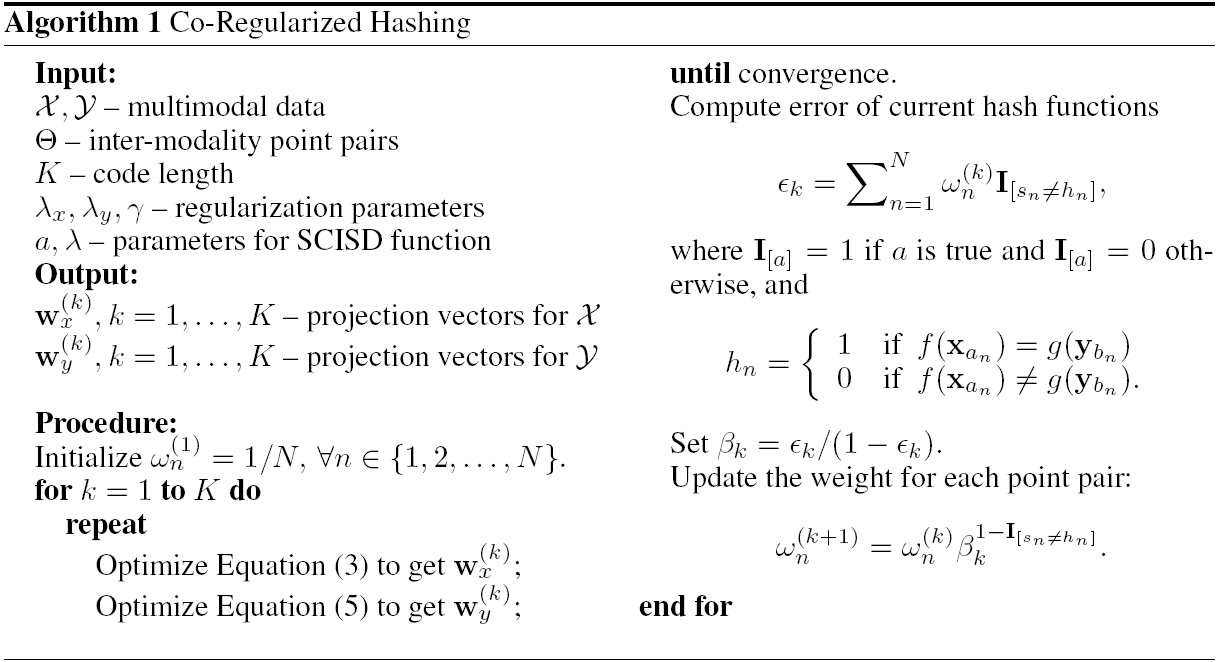
\includegraphics[scale=0.33]{images/algorithm}
\end{frame}

\subsection{Extentions}
\begin{frame}\frametitle{Extentions}
\begin{itemize}
\item Learning nonlinear hash functions via kernel trick:
$w_x=\sum_{i=1}^I\alpha_i\phi_x(x_i)$ and $w_y=\sum_{j=1}^J\beta_j\phi_y(y_j)$
\item Supporting more modalities:
Incorporate loss and regularization term for new modalities and all pairwise loss terms.
\end{itemize}
\end{frame}


%\begin{frame}\frametitle{Pseudo-code of the algorithm}
%\begin{algorithm}[H]
%\KwIn{$A \in \mathbb R^{n \times d},Y \in \mathbb R^{d \times N},\rho$;}
%\KwOut{ID(Y);}
%\emph{Set $B=\left[ A^T,\rho I \right],t=0$}\;
%\emph{Initialize $D_t \in \mathbb R^{(n+d) \times (n+d)}$ as an identity matrix}\;
%\Repeat(\tcp*[h]{Iteratively compute U}){Convergence}
%{
%	Calculate $U_{t+1}=D_t^{-1}B^T(BD_t^{-1}B^T)^{-1}Y$\;
%	Calculate the diagonal matrix $D_{t+1}$,where the i-th diagonal element is $\frac{1}{2\|u_{t+1}^t\|_2}$\;
%	$t=t+1$\;
%}
%\For{$j= 1$ \KwTo $N$}
%{
%	Get $r_s(y_j)=\|y-A^T\delta_s(x_j)\|_2,s=1,2,\cdots ,C$\;
%	$ID(y_i)=\mathop{\min}\limits_{s=1,2,\cdots ,C}r_s(y_j)$\;
%}
%\Return $ID(Y)=((ID(y_1),ID(y_2),\cdots ,ID(y_n))$\;	
%\caption{Classification using $\ell_{2,1}$-norm based regression model}
%\end{algorithm}
%\end{frame}
\end{CJK*}
\end{document}
